Fix inetgers $t, \lambda \geq0$, let $H:\bits^*\to[m]^k$ be a function,  and let
$\Pi = \BF[H,t,\lambda]$ as specified in Figure~\ref{fig:bf}.
%
The possibility of pre-computing the structure in the \errep1 games yields the
following attack. Given a set $\setT\subseteq\bits^*$ of target queries, the
adversary searches for a set $\setR\subseteq\bits^*$ such that
$\Qry^H(\Rep^H(\setR), x) = 1$ for all $x \in \setT$. We call such a set a
\emph{cover} set.
%
Once a suitable~$\setT$ is found, the adversary queries $\REPO(\setR)$ followed
by $\QRYO(x)$ for each $x\in\setT$.
%
Assuming \todo{CP}{Figure out what's needed from the error function in order for
the adversary to succeed with probability~$1$}, the attack succeeds with
probability~$1$.

\cpnote{WIP}





At a high level, the attack works as follows. The attacker chooses a set of~$r$
\emph{target queries} and a set of~$s$ \emph{test queries}.  Its goal is to find
a set~$\col$ of~$n$ test queries for which every target query is a false
positive.
%
It does so by computing the Bloom filter for each subset (by making queries
to~$H$) and evaluating $\Qry$ for each of the target queries (again, using~$H$).
If a satisfying~$\col$ is found, it queries~$\REPO(\col)$ and halts.
%
To finish, it simply queries~$\QRYO$ on each of the target queries and
outputs~$1$. It wins if (and only if)~$\col$ is a satisfying set.
%
The query complexity of this attacker is quite modest; it makes $k(s+r)$ queries
to~$H$, one query to~$\REPO$, and~$r$ queries to~$\QRYO$.  However, since there
are $\binom{s}{n}$ possible sets to check, the runtime of this attack makes it
infeasible, even for modest choices of $k$, $m$, and $n$.
%
In the remainder, we describe a \emph{heuristic} strategy for finding a
satisfying set (if it exists) in which we need only check about $O(kr)$ sets on
average.

Let $\setT = \{x_1, \ldots, x_s\}$ be the set of test queries, and let $\setR =
\{x_{s+1}, \ldots, x_{s+r}\}$ be the set of target queries.
%
Construct a tree whose vertices are labeled with subsets of~$[s]$ as follows:
%
let $\emptyset$ be the root.
%
For each node $I$ and each $w \in [s] \setminus I$, if $\setlen{I} < n$, then let $I
\union \{ w \}$ be a child of~$I$.
%
The new attack works as follows: traverse the tree depth-first, beginning
at~$\emptyset$, until a vertex~$I$ is reached such that each element of $\setR$ is
a false positive for the representation of $\setS_I = \{ x_i : i \in I \}
\subseteq \setT$.
%
Then for every child~$J$ of $I$, the elements of~$\setR$ are false positives
for~$\setS_J$. The adversary may choose any one of these as its query
to~$\REPO$.

The tree has $\binom{s}{n}$ leaves, and it will traverse the entire tree if
there is no solution. Hence, the worst-case runtime is the same as before.
However, we can reduce the search space dramatically in two ways.
%
First, if there is no solution, then often this can be determined without
traversing the tree. Let $M_\setT$ and $M_\setR$ denote the filters
corresponding to the set of test and target queries, respectively.  If for some
$i \in [m]$, the $i$-th bit of $M_\setR$ is set, but the $i$-th bit of $M_\setT$
is not set, then it is immediate that there is no satisfying set.
%
The second is a greedy heuristic for eliminating branches of the search tree.
The idea is that we only take a branch if it results in covering an additional
bit in~$M_\setR$. More precisely, for each child $J$ of~$I$, we do as follows:
if there is a bit~$i$ such that the $i$-th bit of $M_{\col_J}$ and $M_{\setR}$
are set, but the $i$-th bit of~$M_{\col_I}$ is \emph{not set}, then the
branch~$J$ is taken; otherwise it is not.
%
This optimization results in a heuristic attack, since the search may miss the
optimal solution.

We implemented this attack\footnote{The C source code is in a ZIP file
accompanying this submission.} and evaluated its performance.
Figure~\ref{fig:bf-correct-attk-sim} shows the success rate and average number
of sets checked for a number of simulations and various parameters.
%
Unsurprisingly, the success rate decreases as we increase the number of filter
bits (top-left of Figure~\ref{fig:bf-correct-attk-sim}); however, with $k=4$,
$m=1024$, $n=100$, and $r=1$, a test set of just $512$ elements suffices for a
success rate of nearly $60\%$ (top-right). It is also worth noting that
increasing the error parameter only slightly decreases the success rate
(bottom-left). These results show that even for very pessimistic parameter
choices, the classic Bloom filter is not secure in the \errep sense.
%
Finally, we find that the average number of sets that were tested is about
$O(kr)$ within all of the parameter ranges we tested.

%
\newcommand{\mydot}{{\scriptsize\ding{108}}}
\newcommand{\myex}{{\scriptsize\ding{53}}}
\begin{SCfigure*}
\centering
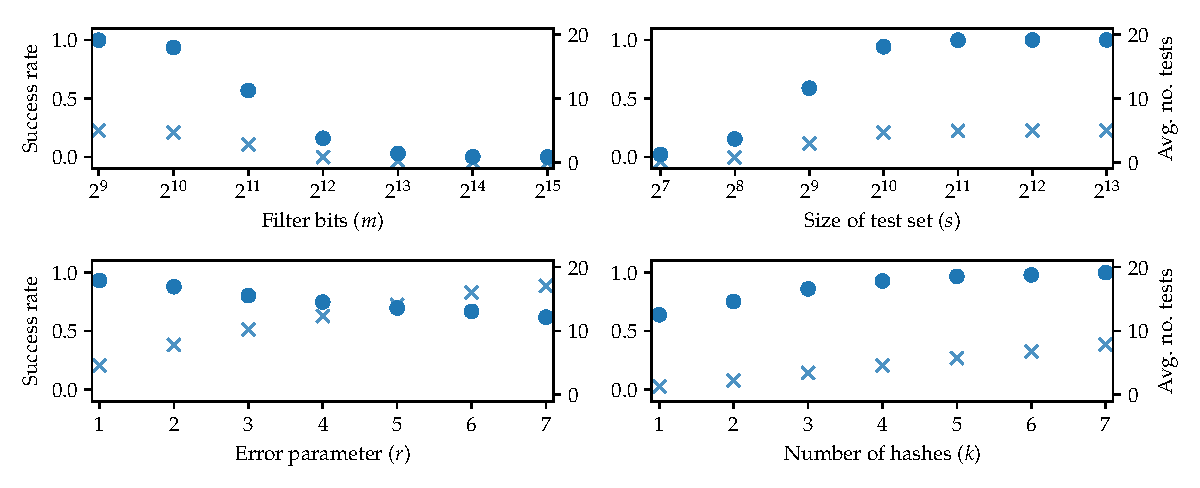
\includegraphics[page=1,scale=0.675]{fig/bf-correct-attk-sim}
\caption{
  %
  Success rate and average-case time complexity for the optimized attack on classic
  Bloom filter.
  %
  Each plot shows the success rate (\mydot), as well as the average number
  of tested sets (\myex), for 1000 executions of
  the attack on simulated inputs.
  %
  Default parameters are $k=4$, $m=2^{10}$, $n=100$, $r=1$, and $s=2^{10}$.
  In each plot, one of these parameters is varied.
}
\label{fig:bf-correct-attk-sim}
\end{SCfigure*}

\heading{Privacy.}
%
\ignore{
  \begin{figure}[t]
    \boxTwoCols{0.48}
    {
      \algorithmv{$\dist[n,\mu]^H$}\\
        $\col \gets \emptyset$;
        for $i\gets 1$ to $n$ do\\
        \tab for $j \gets 1$ to $\mu$ do $\vv_j \gets H(\str(i,j))$\\
        \tab $\col \gets \col \multiunion \{ \str(\vv) \}$\\
        return $\col$
    }
    {
      \adversaryv{$\advA^H$}\\
        for $j \gets 1$ to $\mu$ do $\vv_j \gets H(\str(1,j))$\\
        return $\str(\vv)$\\
    }
    \caption{Distribution~$\dist[n,\mu]$, where $n,\mu \geq0$ are integers, and
    adversary~$\advA$ for attack on ow-rep privacy of~$\BF[k,m,n]$.}
    \label{fig:bf-ow-rep}
  \end{figure}
}
%
The structure~$\BF[k,m,n]$ does not meet our strong notion of \ssrep privacy.
(Indeed, as noted earlier, no keyless data structure can satisfy that
definition.)
%
Even worse, we cannot achieve \owrep privacy for inputs that depend on the
random oracle.
%
Recall that, in the ROM, the distribution~$\dist$ may depend on the random
oracle~$H$.
%
This being the case, we can easily exhibit a distribution with high min-entropy
against which an attacker gets advantage~$1$.
%
Let $\dist$ be a distribution over sets of strings,
parameterized by integers $n,\mu \geq 0$, defined as follows:
%
define a sequence of vectors $\vv_1, \ldots, \vv_n$ so that $\vv_{i}[j] =
H(\str(i,j))$ for each $i\in[n]$ and $j \in [\mu]$.
%
Let $\col = \{\str(\vv_1), \ldots, \str(\vv_n)\}$.
%
Since each query to~$H$ is distinct, the probability that $x \in \col$
for any $x \in \bits^*$ is at most $m^{-\mu}$. Therefore, the point-wise
min-entropy of the distribution is $\mu \cdot \log m$.
%
Now, the attacker can easily compute any $x \in \col$, given access
to~$H$, despite the fact that~$\dist$ has high min-entropy.

Though this attack is theoretical and not particularly interesting in any
practical sense, it is easy to see that \emph{rainbow
tables}~\cite{oechslin2003rainbow}, a practical technique for breaking password
hashes, could be used to deduce the contents.

These negative results for classic BFs in the random oracle model are
reminiscent of the random oracle model \emph{with auxiliary
input}~\cite{unruh2007romaux,dodis2017filling}. In this setting, the adversary
is given a bounded amount of information about the random oracle. This allows us
to model offline computation performed by the adversary before beginning its
attack. Both attacks exploit the fact that the adversary is given the random
oracle \emph{before} choosing its set.

\if{0}{
  \heading{Security of RO-independent collections. }
  %
  \cpnote{I vote for cutting this heading entirely. It feels redundant, and the
  restrictions we need to make on the adversary (no stage-1 RO queries) do not
  seem realistic.}
  %
  Both the correctness and privacy attack exploit the fact that the collection may
  depend on the random oracle.
  %
  We remark that, in both settings, security is achievable for collections chosen
  independently of the RO.
  %For correctness, we do not allow the adversary to make
  %queries to~$H$ in its first stage:
  %
  \begin{theorem}[$\BF$ is correct for RO-independent collections]\label{thm:bf-correct*}
    Fix integers $k,m,n,r\ge0$, let $H \colon \bits^* \to [m]$ be a function, modeled as a
    random oracle, and let $\struct_\bloom = \BF[k,m,n]$.
    %
    Let~$\advA$ be an adversary making~$0$ queries to~$H$ in its first stage, and
    $q_{2} \geq 0$ queries to~$H$ and $q_T \geq 0$ queries to~$\QRYO$ in its
    second stage, such that $q_T + q_2 \geq r$.
    %
    Then
    \[
      \Adv{\errep}_{\struct_\bloom,r}(\advA) \leq
      {\dbinom{q_T + q_{2}}{r}} \left( (1-e^{-kn/m})^k + O(1/m) \right)^r\,,
    \]
    \cpnote{We can't use $\Adv{\errep}_{\struct,r}(t,q_T,q_H)$ notation without
    modification.}\tsnote{Added footnote}\cpnote{Muted footnote}
  \end{theorem}
  %
  To be clear, all of the adversary's RO queries are made in its second
  stage.
  %
  The bound reflects the probability that exactly~$r$ of the adversary's stage-2
  queries are a false positive for the set's representation.
  %
  The proof is technically similar to Theorem~\ref{thm:bf-salt-correct}, and so we
  omit the details.
  %

  For privacy, we must restrict the distribution from making any RO queries.  The
  proof is technically similar to Theorem~\ref{thm:bf-salt-ow-rep}, so we again
  omit the details.

  \begin{theorem}[$\BF$ is ow-rep for RO-independent collections]\label{thm:bf-ow-rep*}
    Fix $k,m,n\geq 0$, let $H \colon \bits^* \to [m]$ be a function,
    and let $\struct_\bloom = \BF[k,m,n]$.
    %
    Then for any $t,q_2,\mu \geq 0$, it holds that
    \[
      \Adv{\owrep}_{\struct_\bloom,\mu}(t,0,q_2) \leq
        \frac{(q_2+1)n}{2^\mu} \,,
    \]
    where~$H$ is modeled as a random oracle.
  \end{theorem}
%
}\fi
